
\chapter*{11 Graphen und Graphenalgorithmen}
\addcontentsline{toc}{chapter}{11 Graphen und Graphenalgorithmen}
\section*{Einführung}
\addcontentsline{toc}{section}{11.1 Einführung}

\begin{itemize}
    \item Entstehung des Graphenformalismus: Königsberger Brückenproblem

    \begin{figure}[htbp]
        \begin{minipage}[t]{8cm}
            \centering
            \vspace{0cm}
            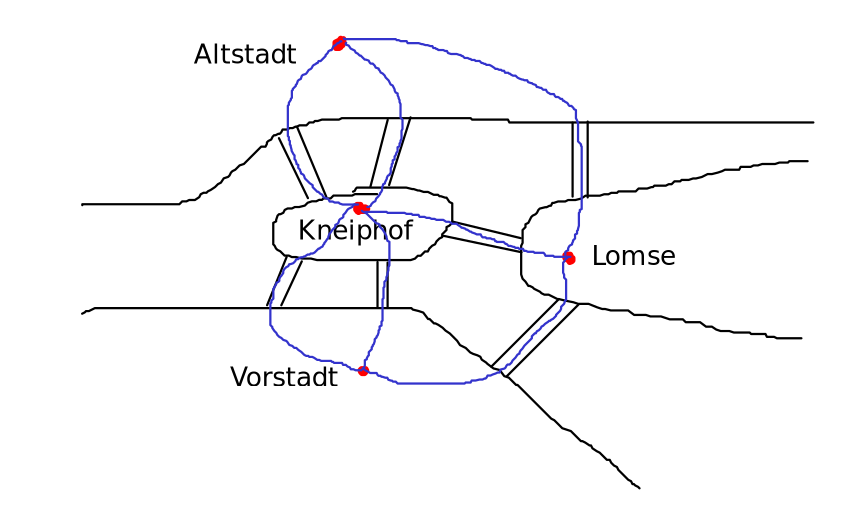
\includegraphics[width=8cm,height=7cm,keepaspectratio]{./Pictures/Koenigsberg.png}\\
            $G = (V, E)$\\
            $E \subset V \times V$
        \end{minipage}
        \begin{minipage}[t]{8cm}
            \vspace{0cm}
            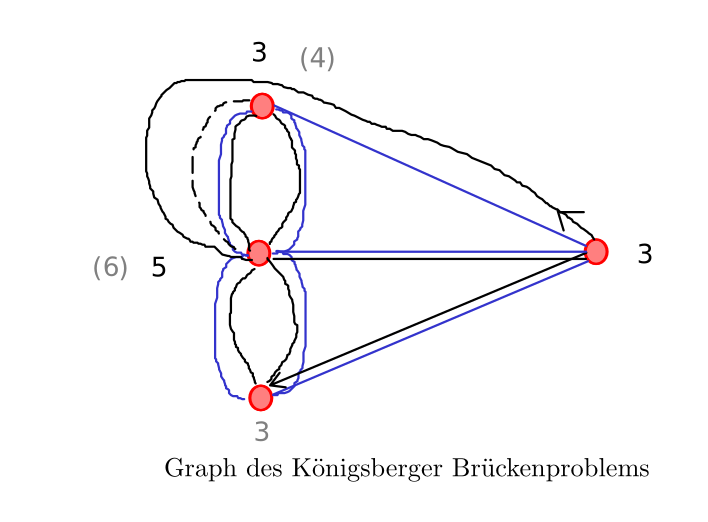
\includegraphics[width=8cm,height=5cm,keepaspectratio]{./Pictures/Brueckengraph.png}\\
            V $\dots$ Vertices, Knoten, E $\dots$ Edges, Kanten\\
            Multigraph $\widehat{=}$ zwei Knoten können durch mehrere Kanten verbunden sein
        \end{minipage}
    \end{figure}

    \item Antwort auf Königsberger Brückenproblem: \glqq Kann man mit einem Spaziergang alle Brücken genau einmal überqueren?\grqq $\Rightarrow$ Nein
    \begin{itemize}
        \item Anforderung: jeder Knoten (Stadtteil), der betreten wird, muss auch wieder verlassen werden $\Rightarrow$ zwei Kanten nötig, oder allg.: eine gerade Anzahl an Kanten
        \item Ausnahmen: Start- und Endpunt des Spaziergangs, falls verschieden
    \end{itemize}
\end{itemize}

\section*{11.2 Definitionen}
\addcontentsline{toc}{section}{11.2 Definitionen}
\begin{itemize}
    \item \textbf{Arten von Graphen}: ungerichtete und gerichtete
    \begin{itemize}
        \item ungerichtet: $u, v \in V \hspace*{1cm} (u,v) \in E \Rightarrow (v, u) \in E$ Kanten ohne Richtung
        \item gerichtet: $u, v \in V \hspace*{1cm} (u,v) \in E \Rightarrow$ $(v, u)$ nicht notwendigerweise vorhanden, zeichne Kanten als \textbf{Pfeile}
        \end{itemize}
        \item \textbf{Grad eines Knotens}:
        \begin{itemize}
        \item ungerichtet: Anzahl der Kanten, die in einem Knoten anliegen, \glqq degree\grqq \\
        $deg(u) = | \{ \ v\  | \ (u,v)\  \in \ E\ \}| \Leftrightarrow (v,u) \in E$
        \item gerichtet:
        \begin{itemize}
            \item in-degree: Anzahl der Kanten, die im Knoten enden
            \item out-degree: Anzahl der Kanten, die im Knoten beginnen
            \item $in\_deg(u) = |\{ \  v \ |\  (v,u) \ \in E\ \}|, \ out\_deg(u) = |\{\  u\  |\  (u,v) \ \in E\ \}|$
        \end{itemize}
        \end{itemize}
            \item vollständiger Graph: alle möglichen Kanten existieren auch, jeder Knoten ist mit jedem Knoten \emph{direkt} verbunden\\
            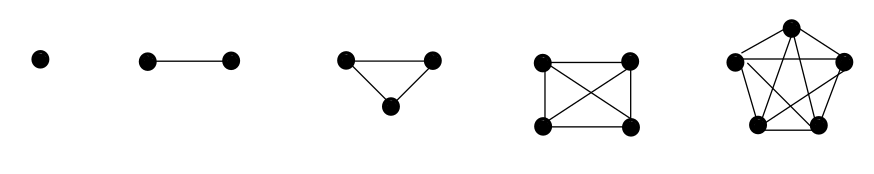
\includegraphics[width=15cm,height=6cm,keepaspectratio]{./Pictures/vollstGraphen.png}\\
            ungerichteter vollständiger Graph: $|E| = \frac{|V|\  ( |V|\  -\ 1)}{2}$\\
            Rätsel: jeder stößt auf Party mit jedem an, es macht 78 mal \glqq pling\grqq \\
            Wie viele Gäste waren da? \hspace*{2cm} $|V| = 13$
            \item Subgraphen: $G' = (V', E')$ ist Subgraph von $G = (V, E)$, wenn :\\ $V'\subseteq V\ ,\  E' \subseteq E$ und für alle $(u, v) \in E'$ muss $(u, v) \in V'$ \\

            Spezialfälle:
            \begin{itemize}
            \item $V' = V$: aufspannender Teilgraph
            \item lösche zuerst Knoten $V' \subset V$, lösche dann alle Kanten \\
            $(u, v)$ wo $u$ oder $v$ $\not \in V'$ $\Rightarrow$ \emph{induzierter Teilgraph}
            \end{itemize}
            \item Wege in Graphen: rekursive Definition
            \begin{itemize}
            \item ein einzelner Knoten $v \in V$ ist ein trivialer Weg der Länge 0
            \item ist eine Folge $(v_1, \cdots, v_{k-1})$ ein Weg und die Kante $(v_{k-1}, v_k)\in E$ existiert, so ist\\ $\underbrace{(v_1, \cdots v_{k-1}, v_k)}_{\text{Länge (k-1)} \widehat{=} \text{Zähle die Kanten im Weg}}$ \hspace*{-1cm}auch ein Weg
            \end{itemize}
            \item Pfad: Weg, wo jeder Knoten \emph{höchstens ein mal} vorkommt ($\widehat{=}$ keine Kreuzungen)
            \item Zyklus: Weg, wo $v_1 = v_k$ Anfangs- gleich Endknoten
            \item Kreis: Zyklus ohne Kreuzung $(v_1, \dots, v_{k-1}, v_k)$ ist Zyklus \\
            d.h. $v_1 = v_k$ und $(v_1, \dots, v_{k-1})$ ist Pfad
            \item Erreichbarkeit $u \rightsquigarrow v$ \hspace{5mm} \glqq v ist erreichbar von u\grqq $\Leftrightarrow$ es gibt einen Weg $(u, \dots, v)$ \\
            $\begin{rcases}
                \text{ungerichtet:} & u \rightsquigarrow v\  \Rightarrow\  v \rightsquigarrow u\\
                \text{gerichtet:} & \text{gilt das nicht unbedingt}
            \end{rcases}$ Konsequenzen für Zusammenhangskomponenten (später)

        \newpage
        \end{itemize}
        \begin{figure}[htbp]
            \begin{minipage}[t]{12cm}
                \vspace{0cm}
                \begin{itemize}
                    \item \textbf{Eulerweg}: enthält jede Kante genau ein Mal \\
                    (Brückenproblem: \glqq Kante\grqq $\widehat{=}$ \glqq Brücke\grqq ) \\
                    Beispiel: Haus vom Nikolaus
                    \item \textbf{Hamiltonweg}: Weg, der alle \emph{Knoten} genau einmal enthält \\
                    Bsp.: Haus vom Nikolaus:
                    \item \textbf{Hamiltonkreis}: Kreis, der alle Knoten genau einmal enthält (außer Anfang/Ende)\\
                    \hspace*{5mm}Bsp.: Haus vom Nikolaus \\
                    Beispiel: Problem des Handlungsreisenden: Suche den kürzesten Hamiltonkreis, der gegebene Städte verbindet $\Rightarrow$ Prototypisches Problem für \emph{NP-vollständig}
                \end{itemize}
            \end{minipage}
            \begin{minipage}[t]{4cm}
                \vspace{-0.5cm}
                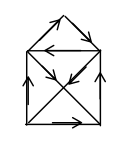
\includegraphics[width=2cm,height=2cm,keepaspectratio]{./Pictures/HausmitPf.png}\\
                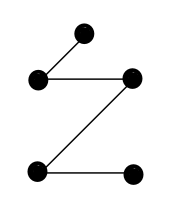
\includegraphics[width=2cm,height=2cm,keepaspectratio]{./Pictures/Hamiltonweg.png}\\
                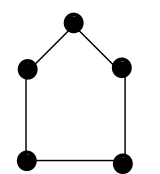
\includegraphics[width=2cm,height=2cm,keepaspectratio]{./Pictures/Hamiltonkreis.png}\\
            \end{minipage}
        \end{figure}

        \section*{11.3 Planare Graphen, ebene Graphen}
        \addcontentsline{toc}{section}{11.3 Planare Graphen, ebene Graphen}
        \begin{itemize}
        \item planar: Graph kann ohne Überkreuzungen in der Ebene gezeichnet werden
        \item eben: wenn tatsächlich so gezeichnet\\
        \includegraphics[width=14cm,height=5cm,keepaspectratio]{./Pictures/plan_ebe_Gr.png}\\
        \begin{figure}[htbp]
            \begin{minipage}[t]{12cm}
                \vspace{0cm}
                \begin{itemize}
                    \item ebener Graph definiert eindeutig Flächen / Regionen in der Ebene
                    \item dualer Graph: jede Region ist ein dualer Knoten\\
                    duale Knoten werden durch Kanten verbunden, wenn die Regionen eine gemeinsame Grenze haben (\emph{nicht nur} gemeinsamen Knoten)
                \end{itemize}
            \end{minipage}
            \begin{minipage}[t]{4cm}
                \vspace{-0.5cm}
                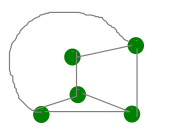
\includegraphics[width=2cm,height=2cm,keepaspectratio]{./Pictures/gruenerGraph.png}\\
            \end{minipage}
        \end{figure}

        Eulersche Gleichung: $|V| - |E| + |F| = 2$
    \end{itemize}
    \begin{itemize}
    \item \textbf{Baum}: \emph{zusammenhängender Graph}, der keine Zyklen enthält \\
    $\forall u,v : u \rightsquigarrow v\  \Rightarrow$ bei $|V|$ Knoten, $|E| = |V| - 1$ Kanten\\
    \begin{flushright}
    \vspace*{-2cm}
    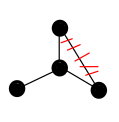
\includegraphics[width=1.5cm,height=1.5cm,keepaspectratio]{./Pictures/Baum_def.png}
    \end{flushright}
    \item \textbf{Spannbaum}: Baum als Subgraph eines Graphen G, der alle Knoten enthält (zusammenhängend $\Leftrightarrow$ G auch zusammenhängend) \\
    \begin{itemize}
        \item Problem: minimaler Spannbaum $\widehat{=}$ kürzeste Kanten $\Rightarrow$ später \\
        \item   wenn G nicht \emph{zusammenhängend}: Wald (hat keine Zyklen) $\widehat{=}$ Menge von Spannbäumen (einer pro Zusammenhangskomponente)
    \end{itemize}
    \end{itemize}

    \section*{11.4 Repräsentation von Graphen}
    \addcontentsline{toc}{section}{11.4 Repräsentation von Graphen}
    \addcontentsline{toc}{subsection}{xx Graphendatenstrukturen, Adjazenzlisten, Adjazenzmatrizen}

    \subsection*{Adjazenzmatrix}
     $ A\  (\ |v|\ \times \ |v|\ )\ :\  a_{i,j} = \begin{cases} 1 & \text{wenn} (u_i, u_j) \in E \\
    0  & \text{sonst}\end{cases}$
    \begin{itemize}
        \item ungerichteter Graph: A immer symmetrische Matrix: $A = A^T$ \\
        \hspace*{1cm} $a_{ij} = a_{ji}$ \hspace*{2mm} weil \hspace*{2mm} $(u_i, u_j) \in E \Rightarrow (u_j, u_i) \in E$
        \item gerichteter Graph: A im allgemeinen nicht symmetrisch
        \item Vorteil:
        \begin{itemize}
            \item man kann in Graphalgorithmen Matrix-Funktionen benutzen
            \item Speicher-effizient für dicht besetzte Graphen $| E | \ \in \bigO{}(|V|^2)$
        \end{itemize}
        \item Nachteil:
        \begin{itemize}
            \item Speicherverschwendung für dünn besetzte Graphen \\
            viele $a_{i,j} = 0$ \hspace*{1cm} $|E| \in \bigO{}(|V|)$ \hspace*{1cm} (z.B. planare Graphen)
        \end{itemize}
    \end{itemize}

    \begin{figure}[htbp]
        \begin{minipage}[t]{4cm}
            \vspace{0cm}
            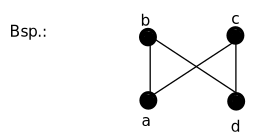
\includegraphics[width=4cm,height=3cm,keepaspectratio]{./Pictures/Adjazenzmatrix.png}
        \end{minipage}
        \begin{minipage}[t]{12cm}
            \vspace{0.0cm}
            $A = \underbrace{\begin{pmatrix}
            0 & 1 & 0 & 1 \\
            1 & 0 & 1 & 0 \\
            0 & 1 & 0 & 1 \\
            1 & 0 & 1 & 0 \\
            \end{pmatrix} }_{a, b, c, d}$ \hspace*{1cm} $al = [[b, d], [a, c], [b, d], [a,c]]$
        \end{minipage}
    \end{figure}

    \subsection*{Adjazenzlisten}
    Array von Arrays: ein Array pro Knoten enthält die Indizes der Nachbarn
    \begin{itemize}
        \item Vorteil:
        \begin{itemize}
            \item speichereffizient für dünn besetzte Graphen ($a_{ij} = 0$ nicht explizit gespeichert), \glqq dünn besetzte Matrixdarstellung\grqq
            \item elegante Schleife über alle Nachbarn und alle Kanten
            \begin{minted}{python}
for node in graph:      #graph = Adjazenzliste
    for neighbor in node:
        #verarbeiten Kante (node, neighbor)
            \end{minted}
        \end{itemize}
        \item Nachteil:
        \begin{itemize}
            \item manche Operationen umständlicher
            \item man muss bei ungerichteten Graphen auf die Symmetrie achten
        \end{itemize}
    \end{itemize}

    \subsection*{Transponierter Graph}
    \begin{itemize}
        \item für alle Kanten: Richtung invertiert \hspace*{1cm} $G^T$
        \item bei ungerichteten Graphen: wieder der gleiche Graph
        \item Adjazenzmatrix: $A_{GT} = A_G^T$
        \item Adjazenzliste:
        \begin{minted}{python}
def transpose_graph(graph):
    gt = [[] for u in graph ]
    for node in range(len(graph)):
        for neighbor in graph[node]:
            gt[neighbor].append(node)
    return gt
        \end{minted}
    \end{itemize}

    \section*{11.5 Iterieren durch Graphen}
    \addcontentsline{toc}{section}{11.5 Iterieren durch Graphen}
    \subsection*{Traversieren von Graphen}
    \begin{itemize}
        \item alle Knoten in einer sinnvollen Reihenfolge (genau einmal) besuchen
        \item Arten:
        \begin{itemize}
            \item Tiefensuche (depth first search, DFS) $\Rightarrow$ erst in die Tiefe, dann zu den anderen Nachbarn
            \item Breitensuche (breadth first search, BFS) $\Rightarrow$ erst zu allen Nachbarn, dann in die Tiefe
        \end{itemize}
    \end{itemize}

    \subsection*{Tiefensuche – DFS}
    \addcontentsline{toc}{subsection}{Tiefensuche, Breitensuche}
    \begin{minted}{python}
def dfs(graph, startnode):           # graph: zusammenhaengenge Adjazenzliste
    visited = [False] * len(graph)   # Flags, welche Knoten schon besucht
    def visit(node):
        if not visited[node]:
            visited[node] = True
            print(node)                  # in der Praxis: anwendungsrelevante Rechnung
            for neighbor in graph[node]: # Adjazenzliste regelt Reihenfolge
                visit(neighbor)
            # print(node)
    visit(startnode)
    \end{minted}

    \newpage
    \begin{figure}[htbp]
        \begin{minipage}[t]{11cm}
            \vspace{0cm}
            \begin{minted}{python}
dfs(graph, 0)
0   #5
1   #6
3   #2
2   #3
5   #4
6   #1
4   #0
=> disovery order / pre-order: verarbeite jeden Knoten VOR seinen Nachbarn -> Hinweg der Rekursion
# => finishing order / post-order: auf dem Rueckweg der Rekursion nach den Nachbarn
            \end{minted}
        \end{minipage}
        \begin{minipage}[t]{6cm}
            \vspace{0.0cm}
            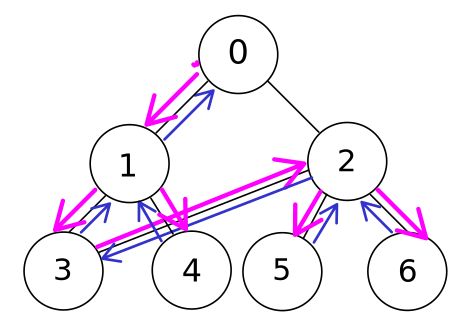
\includegraphics[width=6cm,height=4cm,keepaspectratio]{./Pictures/DFS.png}
        \end{minipage}
    \end{figure}

    \subsubsection*{Anwendungen}
    \begin{figure}[htbp]
        \begin{minipage}[t]{8cm}
            \vspace{0cm}
        \textbf{pre-order traversal}
        \begin{itemize}
            \item Graphen kopieren: kopiere erst den Knoten, dann seine Nachbarn und Kanten
            \item Zusammenhangskomponenten in Graphen finden \\
            (Variante von DFS $\Rightarrow$ später)
            \item wenn Graph schon Baum ist: Abstand jedes Knotens von Wurzel
            \item Taschenrechner (Graph ist Parse tree):\\
            Drucken des Ausdrucks in Funktionsschreibweise  add(3, mul(4,2))
            [Operationsschreibweise: in-order Traversal 3 + (4 * 2)]
        \end{itemize}
        \end{minipage}
        \begin{minipage}[t]{8cm}
        \vspace{0.0cm}
        \textbf{post-order traversal}
        \begin{itemize}
            \item Graphen löschen: erst Nachbarn löschen, dann den Knoten
            \item Bestimme topologische Sortierung eines gerichteten Graphen ($\Rightarrow$ später)
            \item wenn Graph schon Baum ist: Abstand jedes Knotens von den Blättern
            \item Taschenrechner (Graph ist Parse tree):\\
            Auswertung / Berechnung des Ausdrucks
        \end{itemize}
        \end{minipage}
    \end{figure}

    \begin{itemize}
        \item Beides: Weg aus einem Labyrinth $\Rightarrow$ Hausaufgabe\\
        pre-order: Vorwärtsweg \hspace*{1.5cm} $\Leftrightarrow$\hspace*{1.5cm} post-order: Backtracking aus Sackgassen
    \end{itemize}

    Für viele Anwendungen brauchen wir zusätzliche Informationen über den Graphen, die DFS sammeln kann: z.Zt. Flags \emph{visited} \\
    sinnvoll z.B.
    \begin{itemize}
        \item Reihenfolge der Pre- oder Postorder
        \item Elternknoten bei der DFS / von wo wurde node erreicht
    \end{itemize}
    $\Rightarrow$ property maps: Arrays, die für Knoten i und prop[i] die Info speichern

    \subsubsection*{Tiefensuche mit property maps}
    \begin{minted}{python}
def dfs(graph, startnode):
    visited = [False] * len(graph)
    parents = [None] * len(graph)   #zusaetzliche property maps
    disovery_order = []             #
    finishing_order = []            #

    def visit(node, parent):
        if not visited[node]:
            visited[node] = True
            parents[node] = parent
            discovery_order_append(node)
            for neighbor in graph[node]:
                visit(neighbor, node)
            finishing_order.append(node)
    visit(startnode, None)
    return parents, discovery_order, finishing_order
    # Benutze in anderen Algorithmen
    \end{minted}

    Am Beispiel des letzten Graphen:
    parents = [None, 0, 3, 1, 1, 2, 2]\\
    \hspace*{8.3cm} 0, 1, 2, 3, 4, 5, 6\\

    Konvention: Parent des Startnode ist der Startnode selbst $\Rightarrow$ visited Array kann eingespart werden\\


    \subsection*{Breitensuche}
    \begin{minted}{python}
    from collections import deque
    def bfs(graph, startnode):
        parents = [None] * len(graph)
        parents[startnode] = startnode
        q = deque()
        q.append(startnode)

        while len(q) > 0:
            node = q.popleft()                              #q.popright() => Tiefensuche
            print(node)
            for neighbor in graph[node]:
                if parents[neighbor] is None:   #neighbor node nicht besucht
                    parents[neighbor] = node
                    q.append(neighbor)
    \end{minted}

    \begin{figure}[htbp]
        \begin{minipage}[t]{11cm}
        \vspace{0cm}
            \begin{minted}{python}
bfs(graph, 0)
0
1
2
3
4
5
6
=> level order nach Abstand vom startnode und von links nach rechts
            \end{minted}
        \end{minipage}
        \begin{minipage}[t]{6cm}
        \vspace{0.0cm}
        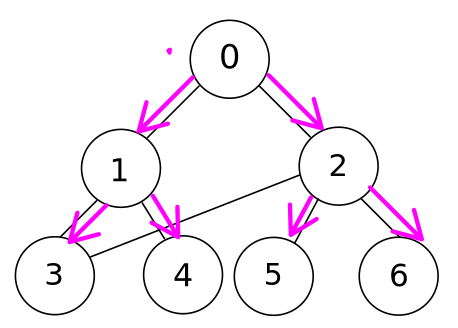
\includegraphics[width=6cm,height=4cm,keepaspectratio]{./Pictures/BFS.png}
        \end{minipage}
    \end{figure}

\newpage
    \subsection*{Anwendungen von Tiefensuche – Damenproblem (beim Schach)}
    \addcontentsline{toc}{subsection}{Damenproblem}
    \textbf{Aufgabe}: Platziere N Damen so auf einem NxN Schachbrett, dass sie sich nicht gegenseitig schlagen\\

    \textbf{Bsp}.: N = 4 \hspace*{1cm}(echte Schachbretter: N = 8)\\ 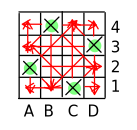
\includegraphics[width=2.5cm,height=2.5cm,keepaspectratio]{./Pictures/Damenbrett.png}\\
    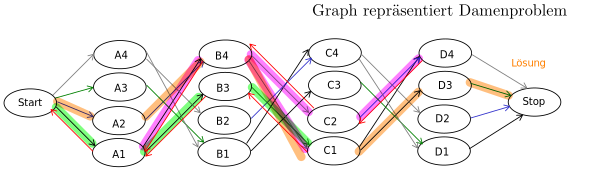
\includegraphics[width=14cm,height=5cm,keepaspectratio]{./Pictures/Damengraph.png}\\

    DFS beginnend bei Start
    \begin{itemize}
    \item checke in discovery\_order, ob Damen sich bis jetzt nicht schlagen können
    \item wenn Test fehlschlägt $\Rightarrow$ backtracking $\widehat{=}$ gehe zurück und probiere den nächsten Nachbarn \\
    \item beim Damenproblem: überprüfe das, indem man den Pfad durch das Parent-Array zurückgeht und den Test mit allen Knoten in dem Pfad ausführt
    \item das erfordert eine adaptive Version von DFS:
    \begin{itemize}
        \item mit parent property map
        \item Kompatibilitätstest der Damen statt print
    \end{itemize}
    \end{itemize}

    \subsection*{Anwendungen der Tiefensuche – Zusammenhangskomponenten}
    \addcontentsline{toc}{subsection}{Zusammenhangskomponenten}
    \begin{itemize}
        \item Bestimmen von Zusammenhangskomponenten: in unzusammenhängendem ungerichtetem Graph:

        \begin{figure}[htbp]
            \begin{minipage}[t]{6cm}
                \vspace{0cm}
                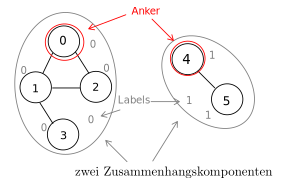
\includegraphics[width=6cm,height=6cm,keepaspectratio]{./Pictures/Zusammenhangskomponenten.png}
            \end{minipage}
            \begin{minipage}[t]{11cm}
                \vspace{0.0cm}
                Definition:
                \begin{enumerate}
                    \item $ u \hspace*{-2cm} \underbrace{\sim}_{\text{\glqq ist äquivalent\grqq \glqq ist in der gleichen Komponente\grqq}}  \hspace*{-2cm} v \hspace*{1cm} \Leftrightarrow \hspace*{1cm} u  \underbrace{\rightsquigarrow}_{\text{es gibt Pfad von u nach v}} v$
                    \item jede Komponente enthält alle von dort erreichbaren Knoten, ist also \emph{maximal} zusammenhängender Subgraph, d.h. wenn man einen weiteren Knoten zum Subgraphen hinzufügt, wäre er nicht mehr zusammenhängend
                \end{enumerate}
            \end{minipage}
        \end{figure}

            \item Idee des Algorithmus:
            \begin{enumerate}
            \item
            \begin{itemize}
            \item definiere für jede Komponente einen \emph{Anker}: ausgezeichneter Knoten, der die Komponente repräsentiert
            \item Konvention: der Knoten mit dem kleinsten Index
            \end{itemize}
            \item starte Tiefensuche von jedem Anker $\Rightarrow$ alle so erreichten Knoten gehören zur selben Komponente
            \item markiere jeden Knoten mit dem Label (laufende Nummer) der jeweiligen Komponente
            \end{enumerate}
            \end{itemize}

            \begin{minted}{python}
def connected_componends(graph):            #graph als Adjazenzliste
    anchors = [None] * len(graph)
    labels = [None] * len(graph)

    def visit(node, anchor):
        if anchors[node] is None:               #node noch nicht besucht
            anchors[node] = anchor                  #anker merken = node als visited markiert
            labels[node] = labels[anchor]
            for neighbor in graph[node]:
                visit(neighbor, anchor)
    current_label = 0                               #label der ersten Komponente
    for node in range(len(graph)):
        if anchors[node] is None:             #neuer Anker gefunden
            labels[node] = current_label
            visit(node, node)                         #Rekursiv alle Knoten der ZK von node besuchen
            current_label += 1
    return anchors, labels
            \end{minted}
            Dieser Algorithmus verwendet das \emph{Anlagerungsprinzip}
            \begin{itemize}
                \item starte von einem Knoten (anchor) und verbinde suksessive alle Knoten der Komponente $\widehat{=}$ wie ein Virus sich ausbreitet
            \end{itemize}
            Gegenteil: \emph{Verschmelzungsprinzip} ($\Rightarrow$ später)\\

            Test, ob ein zusammenhängender Graph ein Baum ist ($\widehat{=}$ ohne Zyklen) oder Zyklen hat
            \begin{itemize}
            \item Definition:
            \begin{itemize}
            \item Baum $\widehat{=}$ es gibt \emph{genau einen} Weg von $u \rightsquigarrow v$ für jedes Paar $u, v \in V$
            \item alternative Wege sind nur bei Zyklen möglich
            \end{itemize}
            \item Idee:
            \begin{itemize}
            \item Tiefensuche: sobald ein Knoten zum zweiten Mal gefunden wird, gab es zwei alternative Wege $\Rightarrow$ Zyklus
            \item Ausnahme: trivialer Zyklus parent $\rightarrow$ node $\rightarrow$ parent darf nicht gewertet werden $\Rightarrow$ Modifikation der Tiefensuche
            \end{itemize}
            \end{itemize}

            \begin{minted}{python}
def undirected_cycle_test(graph):       #graph = zusammenhaengende Adjazenzliste
    visited = [False] * len(graph)
    def visit(node, parent):
        if not visited[node]:
            visited[node] = True
            for neighbor in graph[node]:
                if neighbor == parent:
                    continue                    #trivialen Zyklus ueberspringen
                if visit(neighbor, node):
                    #returns True wenn rekursiv Zyklus gefunden wurde
                    return True
                return False                    #bei "node" kein Zyklus gefunden
        else:
            return True                         #node zum zweiten Mal besucht => Zyklus
    startnode = 0
    return visit(startnode, startnode)
            \end{minted}

        \subsubsection*{Alternativer Algorithmus für Zusammenhangskomponenten: Union-Find}

            \begin{itemize}
                \item wie zuvor: der kleinste Index jeder ZK ist der Anker
                \item aber: Verschmelzungsprinzip:
                \begin{itemize}
                    \item anfangs ist jeder Knoten eine Komponente
                    \item Komponenten schließen sich sukzessive mit ihren Nachbarn zusammen
                    \item wenn kein Zusammenschließen mehr möglich ist $\Rightarrow$ Komponenten sind maximal, also ZK des Graphen
                \end{itemize}
                \item Hilfsfunktion für find-Schritt (Variante 1): \\
                gegeben: node und property map anchors $\Rightarrow$ finde den Anker von node
            \end{itemize}

            \begin{minted}{python}
def find_anchor1(anchors, node):
    while node != anchors[node]:    # Konvention: Anker zeigt in anchors auf sich selbst
        node = anchors[node]        # Kette bis zum Anker verfolgen
    return node                     # jetzt der Anker
            \end{minted}

            \begin{itemize}
                \item Verbesserte Variante 2: Pfadkompression $\widehat{=}$ Verbinde jeden Knoten direkt mit dem Anker $\widehat{=}$ mache aus der Kette einen Stern
            \end{itemize}

            \begin{figure}[htbp]
                \begin{minipage}[t]{11cm}
                    \vspace{0cm}
                    \begin{minted}{python}
def find_anchor(anchor, node):
    start = node
    while node != anchors[node]:
        node = anchors[node]
    anchors[start] = node   #Direktverbindung start->Anker
    return node
                    \end{minted}
                \end{minipage}
                \begin{minipage}[t]{6cm}
                    \vspace{0.0cm}
                    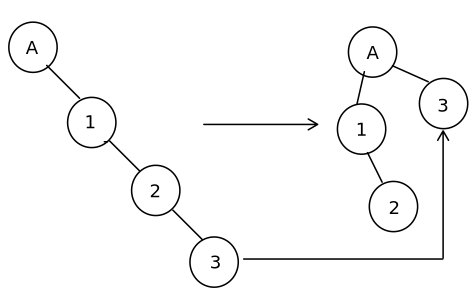
\includegraphics[width=6cm,height=6cm,keepaspectratio]{./Pictures/Stern.png}
                \end{minipage}
            \end{figure}


            Idee:
            \begin{itemize}
                \item Anfangs ist jeder Knoten ein Anker
                \item Iteriere über alle Kanten und verschmelze die Endpunkte (falls sie noch in unterschiedlichen Komponenten sind)
                \item[$\Rightarrow$] wenn alle Kanten abgearbeitet sind $\Rightarrow$ ZK gefunden
                \item Konvention: beim Verschmelzen von zwei Komponenten wird der Anker mit kleinerem Index zum gemeinsamen Anker
                \item betrachte Kanten nur in der Richtung kleiner Index $\rightarrow$ großer Index
            \end{itemize}

            \begin{minted}{python}
def union_find(graph):
    anchors = list(range(len(graph))    #Anfangszustand: jeder Knoten ist Anker anchors[node] == node
    #Komponenten finden
    for node in range(len(graph)):
        for neighbor in graph[node]:
            if neighbor < node: continue    #falsche Kantenrichtung ueberspringen
            a1 = find_anchor(anchors, node)
            a2 = find_anchor(anchors, neighbor)
            if a1 < a2: anchors[a2] = a1
            else: anchors[a1] = a2

    #labels zuweisen
    labels = [None] * len(graph)
    current_label = 0
    for node in range(len(graph)):
        a = find_anchor(anchors, node)
        if a == node:                                   #node ist anchor
            label[a] = current_label
            current_label += 1
        else:
            labels[node] = labels[a]
    return anchors, labels
            \end{minted}
    \begin{center}
        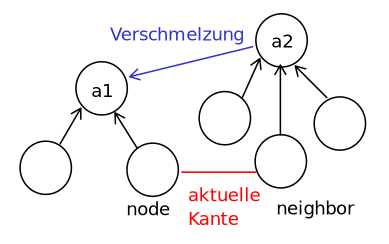
\includegraphics[width=10cm,height=5cm,keepaspectratio]{./Pictures/Verschmelzung.png}
    \end{center}


    \subsection*{Anwendung von Breitensuche – kürzeste Wege}
    \begin{itemize}
        \item ungewichtete Graphen: Länge des Wegen $\widehat{=}$ Anzahl der Kanten \\
        (Gegensatz: gewichtete Graphen: jede Kante hat individuelle Länge)
        \item Idee: property map parents: zeigt für jeden Knoten an, woher man kommt \\
        $\Rightarrow$ Rückverfolgung der Kette parents[target] $\rightarrow$ startnode $\widehat{=}$ kürzester Pfad
        \begin{minted}{python}
from collections import deque

def shortest_path(graph, start, target):
    parents = [None] * len(graph)
    parents[start] = start
    q = deque()
    q.append(start)
    while len(q) > 0:
        node = q.popleft()
        if node == target:
            break               # target gefunden => Schleife beenden
        for neighbor in graph[node]:
            if parents[neighbor] is None:
                parents[neighbor] = node
                q.append(neighbor)
    if parents[target] is None:
        return None     #es gibt keinen Pfad
    #pfad zurueckverfolgen
    pfad = [target]
    while pfad[-1] != start:
        pfad.append(parents[pfad[-1]])
    # Pfad target -> start in start->target umwandeln
    pfad.reverse()
    return pfad
        \end{minted}
    \end{itemize}

    \subsubsection*{Warum findet Breitensuche den kürzesten Weg?}

    \begin{itemize}
        \item BFS besucht Knoten in level-order, als? nach Abstand vom Start
    \end{itemize}
    \begin{figure}[htbp]
        \begin{minipage}{5cm}
            \vspace*{0mm}
            \begin{itemize}
            \item[$\Rightarrow$] Wellenförmige Ausbreitung vom Start
            \item[$\Rightarrow$] sobald die Welle das Ziel erreicht, haben wir den kürzesten Pfad gefunden
            \end{itemize}
        \end{minipage}
        \begin{minipage}{10cm}
            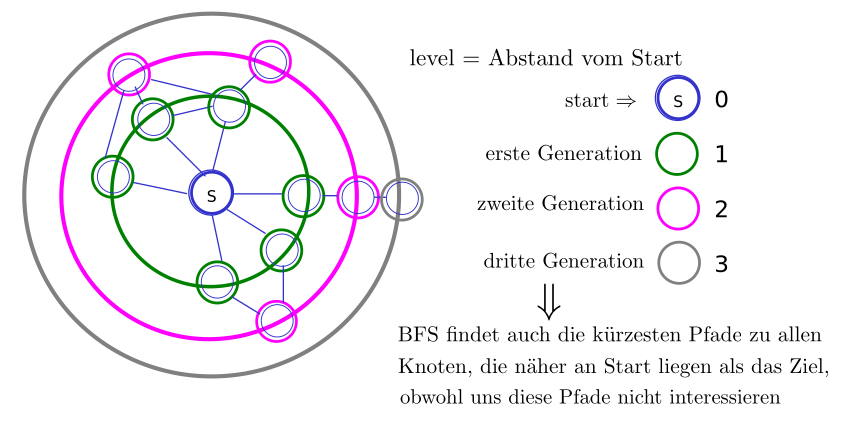
\includegraphics[width=11cm,height=7cm,keepaspectratio]{./Pictures/kurWeg.png}
        \end{minipage}
    \end{figure}

    \section*{11.6 Gewichtete Graphen}
    \addcontentsline{toc}{section}{11.6 Gewichtete Graphen}
        \begin{itemize}
        \item Knotengewichteter Graph: jedem Knoten ist eine Zahl (reell oder ganz) zugeordnet
        \item Kantengewichteter Graph: jeder Kante ist eine Zahl (reell oder ganz) zugeordnet \\
        (gerichtete Graphen: hin- und Rückkante haben im Allgemeinen verschiedene Gewichte)
        \item oder beides gleichzeitig
        \end{itemize}

        \textbf{Beispiele für kantengewichtete Graphen}
        \begin{itemize}
        \item Straßennetzwerke: Gewichte sind Entfernungen oder Fahrzeiten, im Allgemeinen gerichtete Graphen: Einbahnstraßen, Berge
        \item Wechselkurse: (Knoten sind Währungen)
        \item elektrische Netzwerke
        \end{itemize}

        \subsection*{Repräsentation der Gewichte}
        \begin{itemize}
        \item Adjazenzmatrix: $ a_{i, j} \in \{0, 1\} \Rightarrow a_{i, j} = w_{i, j}\hspace*{1cm} (w_{i, j} = 0 \Leftrightarrow (u_i, v_i) \not\in E)$
        \item Property Maps: weights[(i, j)] = $w_{i, j}$
        \end{itemize}

        \textbf{Definition: Kürzester Weg in gerichteten Graphen}
        \addcontentsline{toc}{subsection}{Kürzeste Wege}
        \begin{itemize}
        \item Länge des Weges: [start $= u_0, u_1, \dots, u_{k-1}, u_k$ = target] = P \\
        länge(p) = $\sum\limits_{i=1}^{k} w_{i-1, i}$
        \item kürzester Weg: P(start, target) $\widehat{=}$ Menge aller Wege mit $u_0$ = start, $u_u$ = target, k beliebig \\
        $p^* =$ arg min$_{p \in P\text{(start, target)}}$ länge(p)
        \end{itemize}

        Das Problem unterscheidet sich, wenn es nur positive Gewichte oder positive und negative Gewichte gibt. \\

        Schwierig ist der Fall, wenn es  Zyklen negativer Länge gibt

        \begin{figure}[htbp]
            \begin{minipage}{5cm}
                \begin{flushright}
                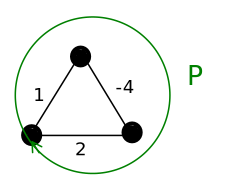
\includegraphics[width=3cm,height=3cm,keepaspectratio]{./Pictures/Dreieckkreis.png}
                \end{flushright}
            \end{minipage}
            \begin{minipage}{10cm}
                länge(p) = -1
                \begin{itemize}[label={$\Rightarrow$}]
                    \item der kürzeste Pfad durchläuft Zyklus unendlich oft
                    \item Gesamtlänge ist $-\infty$
                \end{itemize}
            \end{minipage}
        \end{figure}

        $\Rightarrow$ Bellmann-Ford Algorithmus: bricht Suche ab, wenn negativer Zyklus gefunden, sonst findet er den kürzesten Pfad
        \begin{figure}[htbp]
            \begin{minipage}{8cm}
                \begin{itemize}
                    \item Vorteil: negative Gewichte erlaubt
                    \item Nachteil: langsamer
                    \item Beispiel: Arbitrage-Geschäfte
                \end{itemize}
            \end{minipage}
            \begin{minipage}{5cm}
                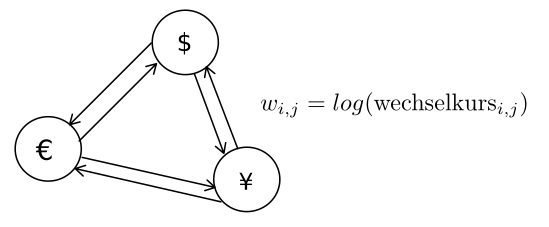
\includegraphics[width=7cm,height=4cm,keepaspectratio]{./Pictures/Wechselkurs.png}
            \end{minipage}
        \end{figure}

        \addcontentsline{toc}{subsection}{Dijkstra-Algorithmus}
        \begin{itemize}
        \item wenn alle $w_{i, j} > 0$: \emph{Algorithmus von Dijkstra} , Komplexität $\bigO{}(|E| * log|V|)$ \\
        \textbf{Idee}: Verwende statt einer Queue (in BFS) eine priority queue \\
        $\Rightarrow$ expandiere kurze Wege zuerst
        \begin{minted}{python}
import heapq
# Konvention: MinHeap ist ein Python-Array (list),
# Elemente sind Tupel(priority, data1, data2, ...) (Anwendungsdaten)

def dijkstra(graph, weights, start, target):
    parents = [None] * len(graph)
    q = []
    #Heap statt Deque
    heapq.heappush[q, (0.0, start, start))        # Prioritaet, aktueller Knoten, parent
    while len(q) > 0:
        length, node, parent = heapq.heappop(q)
        # Knoten nicht zweimal besuchen
        if parents[node] is not None:
            continue  # wir kennen bereits kuerzeren Weg
        parents[node] = parent
        if node == target: break                  # Ziel gefunden
        for neighbor in graph[node]:
            # kuerzester Weg zu neighbor noch nicht bekannt
            if parents[neighbor] is None:
            # Prioritaet / Laenge berechnen
            new_length = length + weight[(node, neighbor)]
            heapq.heappush(q, (new_length, neighbor, node))
    if parents[target] is None: return None, None
    path = [target]
    while path[-1] != start:
    path.append(parents[path[-1]])
    path.reverse()
    return path, length
        \end{minted}
        \end{itemize}

        \subsubsection*{Komplexität vom Dijkstra-Algorithmus}
        \begin{itemize}
        \item while len(q) $>$ 0: \\
        ... \#1 \hspace*{6cm} \textcolor{red}{\#heappop(q): $\bigO{}(log(len(q)))$}\\
        if parents[node] is not None: continue \textcolor{red}{$\Leftarrow$ jeder Knoten wird höchstens einmal expandiert}\\
        parents[node] = parent \\
        ... \#2\hspace*{6cm}  \textcolor{red}{\#für jeden Knoten höchstens 1-mal}
        \item jede Kante kann höchstens zweimal gefunden werden: (u,v) und (v, u), weil jeder Anfangsknoten nur einmal expandiert \\
        tatsächlich wird \emph{jede Kante nur einmal gefunden}, weil wir Kanten überspringen, deren Endknoten schon expandiert wurde
        \item[$\Rightarrow$] im Heap liegen Kanten, d.h. len(q) $\in \bigO{}(|E|)$ \\
        Komplexität des Heap-Zugriffs: \hspace*{0.5cm} $\bigO{}(log|E|)$
        \item in gewöhnlichen Graphen (zw. zwei Knoten höchstens eine Kante): \hspace*{0.5cm} $|E| \in \bigO{}(|V|^2)$
        \item max $|E|$ Durchläufe durch die while-Schleife
        \item[$\Rightarrow$] insgesamt: Komplexität \hspace*{0.5cm} $\bigO{}(|E| * log|E|) \ =\  \bigO{}(|E| log |V|^2) \ =\  \bigO{}(|E| log |V|)$
        \end{itemize}

        \subsubsection*{Korrektheit: Findet Dijkstra wirklich den kürzesten Pfad?}

        \textbf{Beobachtung}: length wird in der nächsten Iteration der while-Schleife nie kürzer
        \[ length_{i-1} \geq length_i\]

        \textbf{Beweis}:(indirekt) Angenommen, $l_{i+1} < l_i$ und $l_{i+1}$ ist Top-Element in Iteration i
        \begin{itemize}
            \item Fall 1: Der Weg der Länge $l_{i+1}$ war schon in Iteration i bekannt $\Rightarrow$ $l_i$ war nicht Top in Iteration i$\Rightarrow w!$
            \item Fall2: Der Weg der Länge $l_{i+1}$ wurde in Iteration i entdeckt. $l_{i+1} = l_i + w_{uv} > l_i \Rightarrow w!$\\
        \end{itemize}

        \textbf{Korrektheitsbeweis}(indirekt):
        \begin{itemize}
            \item Annahme: Dijkstra: node $\rightarrow$ parent $\rightsquigarrow$ start \hspace*{1.2cm} $l$\\
            wirklicher kürzester Weg: node $\rightarrow$ x $\rightsquigarrow$ start \hspace*{1cm} $l' < l$\\
            In Iteration i war node $\rightarrow$ parent das Top-Element des Heaps, aber
            \item Fall 1: x $\rightsquigarrow$ start ist auch schon im Heap \\
            wenn x $\rightsquigarrow$ start kürzer ist als node $\rightsquigarrow$ start, hätte er schon früher Top-Element sein müssen $\rightarrow w!$
            \item Fall 2: x $\rightsquigarrow$ start war noch nicht im Heap $\Rightarrow$ länge (x $\rightsquigarrow$ start) ist wegen der Monotonie von length nicht kürzer als $l$\\
            also ist $l'$= length (node $\rightarrow x \rightsquigarrow$ start) = $\underbrace{\text{length}(x \rightsquigarrow \text{start})}_{> l \  \Rightarrow \ w!} + \underbrace{w_{x, node}}_{>0}$
        \end{itemize}

        \subsubsection*{Induktiver Beweis für alle Iterationen:}
        \textbf{Induktionsanfang}: Weg start $\rightarrow$ start $\widehat{=}$ Länge 0 $\Rightarrow$ kürzester Pfad, Fall target = start\\

        \textbf{Induktionsschritt}: wir kennen den kürzesten Weg zu allen Knoten mit Länge $\leq l$ (= Länge (node $\rightarrow$ parent $\rightsquigarrow$ start)\\
        dann ist das nächste Top-Element (node $\rightarrow$ parent $\rightsquigarrow$ start) der kürzeste Weg für node $\rightsquigarrow$ start (s.o.) \\

        \textbf{Induktionsende}:Sobald das Top-Element (target $\rightarrow$ parent $\rightsquigarrow$ start) ist haben wir den kürzesten Weg target $\rightsquigarrow$ start gefunden\\

        \textbf{Konsequenz}: Dijkstra findet auch alle kürzesten Wege, die kürzer als target $\rightsquigarrow$ start sind (wie Breitensuche), kann ineffizient sein\\

        \textbf{Bsp.:} Weg von Frankfurt(Main) $\rightsquigarrow$ Dresden (460 km)\\
        \hspace*{0.5cm} findet auch die kürzesten Wege Frankfurt $\begin{rcases}\rightsquigarrow \text{Stuttgart(210 km)} \\ \rightsquigarrow
        \text{Dortmund(220 km)} \end{rcases}$ ignorieren\\

        \hspace*{0.5cm} aber: kürzesten Wege Frankfurt $\begin{rcases} \rightsquigarrow \text{Erfurt (260km)} \\
        \rightsquigarrow \text{Suhl (210km)} \end{rcases}$ nicht ignorieren \\
        \hspace*{0.5cm} könnten Teil des Weges Fr $\rightsquigarrow$ Dresden sein\\

        Wie entscheiden wir, welche Wege ignoriert werden dürfen?


        \subsection*{A* – Algorithmus}
        \addcontentsline{toc}{subsection}{A* – Algorithmus}
        \begin{itemize}
            \item benötigt Schätzfunktion für die Restentfernung guess(Zwischenziel, target)
            \item Trick: ändere Prioritaet von length nach length + guess
            \item Voraussetzung: length(Zwischenziel, target) $\geq$ guess(Zwischenziel, target)\\
            Dann ist garantiert, dass immernoch der Korrekte kürzeste Pfad gefunden wird:
            \begin{itemize}
                \item nur erfüllbar, wenn 0 = length(target, target) = guess(target, target)\\
                $\Rightarrow$ Target wird mit der gleichen Länge zum Top-Element wie bei Dijkstra
                \item für alle Zwischenziele auf dem wahren kürzesten Weg gilt:\\ \hspace*{0.5cm} length(zwischen, start) + guess(zwischen, target) $\leq$ length(target, start)\\
                $\Rightarrow$ alle Zwischenziele waren Top-Elemente vor target und wurden bereits expandiert $\widehat{=}$ man ignoriert nie die korrekten Zwischenziele
                \item aber: Zwischenziele mit length(zwischen, start) + guess(zwischen, target) $>$ length(target, start) werden ignoriert, $\Rightarrow$ $A^*$ effizienter als Dijkstra
            \end{itemize}
        \end{itemize}

    \subsubsection*{Beispiel für kürzester Weg mit Dijkstra und A*}

    \begin{figure}[htbp]
        \begin{minipage}{2.5cm}
            \vspace*{0mm}
            \textbf{Dijkstra}
            \begin{tabular}{L{1cm} | L{1.5cm}}
                Prio & Pfad \\ \hline
                0 & S\\
                2 & SA \\
                3 & SC \\
                6 & SAB \\
                8 & SCB \\
                9 & SCF \\
                12 & SCDE \\
                16 & SABG \\
                \colorbox{green}{18} & \colorbox{green}{SCDET} \\
                21 & SCFT \\
                26 & SABGT \\
            \end{tabular}
        \end{minipage}
        \begin{minipage}{8cm}
            \vspace*{0mm}
            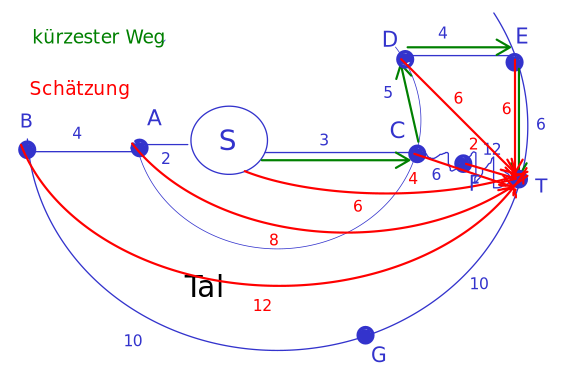
\includegraphics[width=7cm,height=5cm,keepaspectratio]{./Pictures/Banane.png}
        \end{minipage}
        \begin{minipage}{4cm}
            \vspace*{0mm}
            \textbf{A$^*$}
            \begin{tabular}{L{2cm} | L{2cm}}
                Prio & Pfad \\ \hline
                6 = 0 \textcolor{red}{+ 6} & S\\
                7 = 3 \textcolor{red}{+ 4} & SC \\
                10 = 2 \textcolor{red}{+ 8}  & SA\\
                11 = 9 \textcolor{red}{+ 2}  & SCF \\
                14 = 8 \textcolor{red}{+ 6}  & SCD \\
                18 = 12 \textcolor{red}{+ 6}  & SCDE \\
                18 = 6 \textcolor{red}{+ 12}  & SAB \\
                21 = 21 \textcolor{red}{+ 0}  & SCFT \\
            \end{tabular}
            \colorbox{green}{18 = 18  \textcolor{red}{+ 0} \hspace*{0.5cm} SCDET}
        \end{minipage}
    \end{figure}


    \subsection*{Minimaler Spannbaum} (minimum spanning tree, MST)\\
    \addcontentsline{toc}{subsection}{Minimaler Spannbaum}

    \textbf{Definition}: gewichteter ungerichteter Graph $G = (V, E, w)$ zusammenhängend\\
    \begin{itemize}
        \item gesucht: $G' = (V, E' \subset E, w' \subset w)$, so dass $\sum\limits_{l = E'} we' \rightarrow$ \emph{minimal} und G' zusammenhängend
        \item \glqq Spann\grqq: V' = V
        \item \glqq Baum\grqq : G' ist immer ein Baum. Hätte G' ein Zyklus, könnten wir eine Kante im Zyklus löschen, ohne den Zusammenhang zu stören, und dabei die Summe $\sum\limits_{l=E'}we'$ verringern
    \end{itemize}

    \textbf{Variante}: ist G nicht zusammenhängend\\
    \hspace*{1cm} $\Rightarrow$ minimaler Spannbaum für jede Komponente $\Rightarrow$ Wald von minimalen Bäumen\\

    \textbf{Beispiel:}
    \begin{figure}[htbp]
        \begin{minipage}{5cm}
            \vspace*{0cm}
            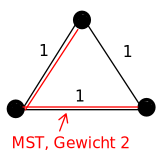
\includegraphics[width=5cm,height=3cm,keepaspectratio]{./Pictures/MSTrot.png}
            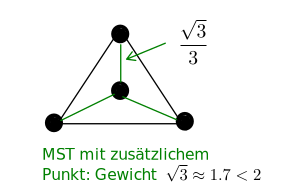
\includegraphics[width=5cm,height=3cm,keepaspectratio]{./Pictures/MSTgruen.png}
        \end{minipage}
        \begin{minipage}{10cm}
            \vspace*{0cm}
            \textbf{Beobachtung}: Wenn man neue Knoten hinzufügen darf, kann der neue Spannbaum kürzer sein als der alte (\glqq Steiner Punkte\grqq)\\

            \textbf{Anwendung}: Eisenbahnknoten\\
            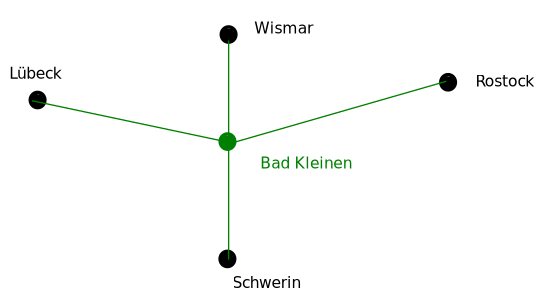
\includegraphics[width=8cm,height=5cm,keepaspectratio]{./Pictures/Bahn.png}\\
            Im MST-Problem ist das Hinzufügen neuer Punkte nicht erlaubt.
        \end{minipage}
    \end{figure}

    \subsubsection*{Algorithmen: Prim(Anlagerungsprinzip), Kruskal (Verschmelzungsprinzip)}
    \addcontentsline{toc}{subsubsection}{Algorithmen: Prim, Kruskal}

    \textbf{Prim:} \begin{itemize}
        \item starte mit einem beliebigen Knoten und füge den Knoten mit der kürzesten Kante hinzu, solange dadurch kein Zyklus entsteht, andernfalls ignoriere die Kante
        \item Algorithmus entspricht Tiefensuche und Breitensuche\\
        Datentruktur: Stack(letzten expandieren) und Queue(ältesten expandieren), Prim: Heap(nächsten Knoten expandieren)
    \end{itemize}

    \begin{minted}{python}
import heapq

def prim(graph, weights):                   #Adjazenzliste, Property map
    parents = [None] * len(graph)
    q = []
    heapq.heappush(q, (0.0, 0, 0))      #Prioritaet, start, parent
    sum = 0.0
    while len(q) > 0:
        w, node, parent = heapq.heappop(q)
        # Knoten zweimal besuchen = Zyklus => ueberspringen
        if parents[node] is not None:
            continue
        parents[node] = parent
        sum += w
        for neighbor in graph[node]:
            if parents[neighbor] is None:
                heapq.heappush(q, (weights[(node, neighbor)], neighbor, node))#prio,node,parent
    return parents, sum
    \end{minted}

    \textbf{Kruskal:}
    \begin{itemize}
        \item Anfangs ist jeder Knoten ein Baum für sich, in jeder Iteration werden die Teilbäume mit der kürzesten Kante verschmolzen, beachte:\\
        dabei nur Kanten benutzen, deren Enden in verschiedenen Bäumen liegen, die anderen werden übersprungen, weil Zyklus entstehen würde
        \item zweckmäßig: Kanten anfangs nach Priorität sortieren
    \end{itemize}

    \begin{minted}{python}
def kruskal(graph, weights):
    anchors = list(range(len(graph)))   # wie bei union-find
    results = []                        # enthaelt spaeter die Kanten des Baums
    q = []
    sum = 0.0
    for edge, w in weights.items():     # edge:(u,v)
        heap.heappush(q, (w, edge))
    while len(q) > 0:
        w, edge = heapq.heappop(q)
        a1 = find_anchor(anchors, edge[0])
        a2 = find_anchor(anchors, edge[1])
        #if w > w_max: break    => Clusterung
        if a1 != a2:                     # u und v in verschiedenen Teilbaeumen
            anchors[a2] = a1             # Teilbaeume verschmelzen
            result.append(edge)
            sum += w
    return results, sum
    \end{minted}

    \textbf{Komplexität}: Heap enthält maximal $|E|$ Elemente $\Rightarrow$ Zugriff $\bigO{}\ (log|E|)$\\
    insgesamt: $\bigO{}\ (|E|\ log|E|) = \bigO{}\ (|E| \ log |V|)$ weil $|E| \in \bigO{}\ (|V|)$\\

    \textbf{Anwendung von Kruskal-Alg. zur Bestimmung von Datenclustern}\\
    \begin{figure}[htbp]
        \begin{minipage}{8cm}
            \vspace*{0mm}
            vollständiger Graph mit $w_{u,v}$ = dist(u, v)\\

            im MST gibt es zwei Arten von Kanten:
            \begin{itemize}
                \item kurze $\widehat{=}$ innerhalb der Cluster
                \item lange $\widehat{=}$ zwischen Clustern
                \item[$\Rightarrow$] lange Kanten löschen
            \end{itemize}
        \end{minipage}
        \begin{minipage}{8cm}
            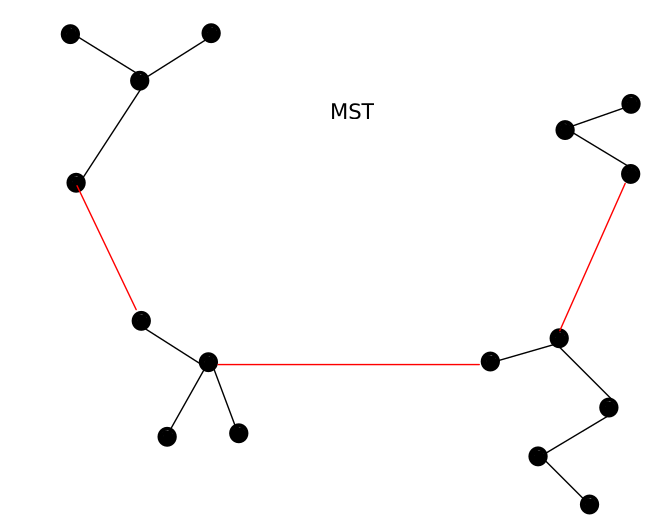
\includegraphics[width=8cm,height=4cm,keepaspectratio]{./Pictures/Sternbild.png}
        \end{minipage}
    \end{figure}
    \begin{itemize}
        \item[$\Rightarrow$] unzusammenhängender Graph $\Rightarrow$ Zusammenhangskomponenten sind Cluster $\widehat{=}$ Gruppen von Knoten, die sich nahe sind, während die Clusterzentren größeren Abstand haben
    \end{itemize}

    \textbf{mit Kruskel}: neuen Funktionsparameter $w_{max}$ übergeben, so dass
    \[w \leq w_{max} \widehat{=}\text{ \glqq kurz\grqq},\hspace*{1cm} w > w_{max} \widehat{=} \text{\glqq lang\grqq} \]
    Schleife über sortiere Kanten abbrechen, sobald $w > w_{max}$
    \begin{figure}[htbp]
        \begin{minipage}{8cm}
            \vspace*{0mm}
            \begin{itemize}
                \item \glqq Single linkage Clustering\grqq
                \item schwierig: Bestimmung des richtigen $w_{max}$
            \end{itemize}
        \end{minipage}
        \begin{minipage}{8cm}
            \vspace*{0mm}
            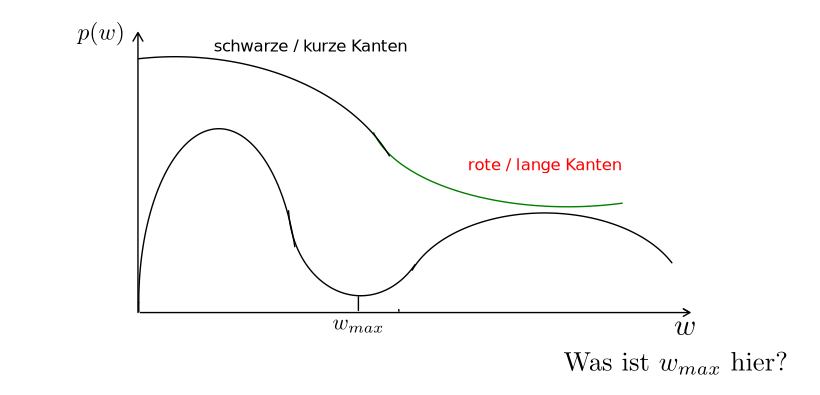
\includegraphics[width=8cm,height=4cm,keepaspectratio]{./Pictures/wGraph.png}
        \end{minipage}
    \end{figure}


    \section*{11.7 Algorithmen für gerichtete Graphen}
    \addcontentsline{toc}{section}{11.7 Algorithmen für gerichtete Graphen}

    Anwendungen gerichteter Graphen:
    \begin{itemize}
        \item Straßenbahnnetzwerke mit Einbahnstraßen und/oder unterschiedlichen Entfernungen / Fahrzeiten für hin vs. zurück
        \item Abhängigkeitsgraphen:
        \begin{itemize}
            \item welche Aktion muss man vor einer anderen Aktion ausführen
            \item zeitliche Beziehung \hspace*{1cm}past $\rightarrow$ present $\rightarrow$ future
            \item kausale Abhängigkeiten \hspace*{0.1cm} Ursache $\rightarrow$ Wirkung
            \item Softwareabhängigkeiten: Python-Modul import json importiert zuerst \emph{decimal}, das wiederum \emph{copy} und \emph{collections}, danach \emph{json.encoder} und \emph{json.decoder}, die wiederum \emph{re} und \emph{sys}
        \end{itemize}
        \item Internet: Hyperlinks sind gerichtet
    \end{itemize}

    \textbf{Anwendung: sequence alignment}
    \begin{itemize}
        \item verschiedene Sequenzen des gleichen Phänomens, die nicht exakt gleich ablaufen, so gegeneinander verschieben / skalieren (linear alignment), dass korrespondierende Ereignisse übereinander liegen
        \item oder nicht-linear verzerren
        \item Bsp.: EKG
    \end{itemize}

    \subsection*{Anwendung von sequence alignment : \emph{edit distance}}
    \begin{itemize}
        \item Schreibprogramm mit Rechtschreibprüfung, getippt wurde \glqq TPE\grqq
        \item Welches Wort könnte gemeint sein (zur Anzeige im Kontextmenü)?
        \item Welches Wort ist ähnlich? $\Rightarrow$ Wie viele Editieroperationen sind nötig, um \glqq TPE\grqq \ in ein sinnvolles Wort zu überführen? \emph{edit distance}
        \item zwei erlaubte Operationen:
        \begin{itemize}
            \item \textcolor{magenta}{ein Jokerzeichen einfügen} (Kosten a)
            \item \textcolor{red}{einen Buchstaben tauschen} (Kosten b)
        \end{itemize}
        \item sinnvolles Wort: \glqq TOPF\grqq , mögliche Alignments:
    \end{itemize}
    \[ \underbrace{\begin{matrix}
    T & O & P & \textcolor{red}{F} \\
    T & \textcolor{magenta}{?} & P & \textcolor{red}{E}
    \end{matrix}}_{\text{\textcolor{red}{Kosten a + b}}}\hspace*{0.8cm}  \underbrace{\begin{matrix} T & O & P & F & ? & ? & ? \\ ? & ? & ? & ? & T & P & E \end{matrix}}_{\text{7 * a}} \hspace*{0.8cm} \underbrace{\begin{matrix} T & O & P & F \\ T & P & E & ? \end{matrix}}_{\text{\textcolor{magenta}{a + 2*b}}} \hspace*{0.8cm} \text{usw.\\ edit dist } \widehat{=} \text{ minimum der Kosten}\]

    \begin{itemize}[label={}]
        \item Aufgabe: finde sequence alignment, das die Kosten minimiert.
        \item Lösung: Dijkstra-Algorithmus auf gerichtete und gewichtete Graphen
    \end{itemize}

    \begin{figure}[htbp]
        \begin{minipage}{5cm}
            \vspace*{0mm}
            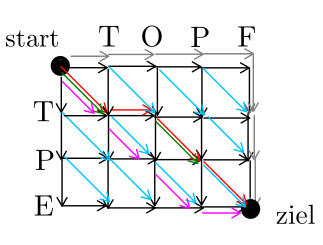
\includegraphics[width=5cm,height=4cm,keepaspectratio]{./Pictures/Dijkstragitter.png}
        \end{minipage}
        \begin{minipage}{10cm}
            \vspace*{0mm}
            Bedeutung der Kanten:
            \begin{itemize}
                \item $\rightarrow$ Joker im linken Wort einfügen
                \item $\downarrow$ Joker im rechten Wort einfügen (Kosten a)
                \item \textcolor{green}{$\searrow$} zwei Buchstaben matchen und passt (Kosten 0)
                \item \textcolor{cyan}{$\searrow$} zwei Buchstaben matchen und tauschen (Kosten b)
            \end{itemize}
            Optimale Lösung: kürzester Weg Start $\rightarrow$ Ziel
        \end{minipage}
    \end{figure}

    \subsection*{Anwendung: Abhängigkeitsgraph}

    Welche Aktion muss man vor einer anderen Aktion ausführen? \\

    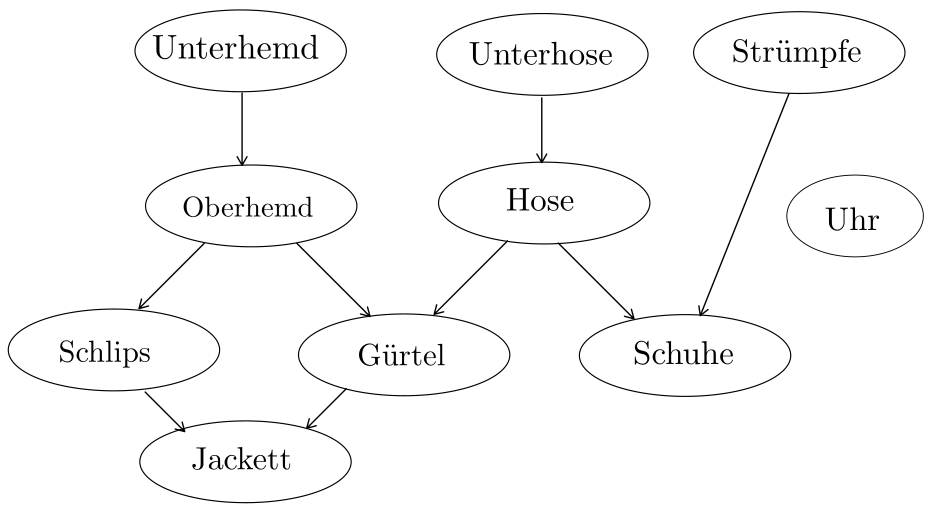
\includegraphics[width=10cm,height=7cm,keepaspectratio]{./Pictures/Anziehen.png}\\
    Azyklischer gerichteter Graph (Zyklus $\widehat{=}$ Anziehen wäre unmöglich) \\
    DAG: directed acyclic graph\\

    \textbf{Satz}: Jeder DAG definiert eine Halbordnung:
    \[ x \leq y \hspace*{5mm}\text{ (Reflexivität)}\]
    \[ x \leq y \land y \leq x \Rightarrow x = y\hspace*{5mm} \text{ (Antisymmetrie)}\]
    \[ x \leq y \land y \leq z \Rightarrow x \leq z \hspace*{5mm} \text{(Transitivität)}\]

    \begin{itemize}[label={}]
        \item bei Totalordnung zusätzlich: $x\leq y$ oder $y \leq z$ ist wahr, es gibt Kante (x,y) oder (y, z)
        \item   bei Halbordnung: $x \leq y \Rightarrow$ \glqq unknown\grqq , falls x und y nicht vergleichbar $\widehat{=}$ keine Kante (x, y) oder (y, z)
    \end{itemize}



    \textbf{Aufgabe}: \emph{Topologische Sortierung}, d.h. Totalordnung, die die Halbordnung enthält\\

    Idee der topologischen Sortierung ein DAG: Weise jedem Knoten eine Zahl $0, 1, \dots, N-1$ zu, sodass die Ordnung dieser Zahlen die Halbordnung enthält, d.h. wenn wir den Graphen auf eine Gerade zeichnen, gehen alle Kanten nach rechts (falls (x, y) als $x \leq y$ true interpretiert wird)\\

    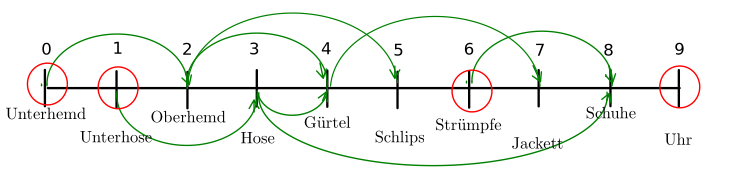
\includegraphics[width=12cm,height=4cm,keepaspectratio]{./Pictures/Zeitstrahl.png}\\

    \textbf{Beobachtungen}:
    \begin{itemize}
        \item es gibt viele erlaubte Totalordnungen
        \item wichtig sind die Knoten \emph{ohne} eingehende Pfeile \textcolor{red}{(0, 1, 6, 9)}
    \end{itemize}

    Lösung 1:
    \begin{enumerate}
        \item Suche Knoten mit Eingangsgrad 0 und setze ihne an die nächste freie Position
        \item entferne diesen Knoten aus dem Graphen inkl. seiner ausgehenden Kanten\\
        $\Rightarrow$ dadurch verringert sich der Eingangsgrad seiner Kinder
        \item gehe zu 1.
    \end{enumerate}
    \begin{itemize}[label={}]
        \item wenn es keine Knoten mit Eingangsgrad 0 mehr gibt, aber noch nicht alle Knoten platziert wurden, ist der Graph zyklisch $\Rightarrow$ keine topologische Sortierung möglich
    \end{itemize}


    \begin{minted}{python}
def topological_sort(graph):
    in_degree = [0] * len(graph)
    for node in range(len(graph)):
        for neighbor in graph[node]:
            in_degree[neighbor] += 1
    result = [] #result[node] -> Position von node auf der Geraden
    for node in range(len(graph)):
        if in_degree [node] == 0:
            result.append(node)
    k = 0
    while k < len(result):
        node = result[k]
        k += 1
        for neighbor in graph[node]:
            in_degree[neighbor] -= 1
            if in_degree[neighbor] == 0:
                result.append(neighbor)
    if len(result) == len(graph): # alle Knoten eingefuegt
        return result
    else:                         # Zyklus
        return None
    \end{minted}


    Lösung 2: die reverse post-order (finishing order von Tiefensuche rückwärts) eines DAGs ist eine topologische Sortierung

    \begin{minted}{python}
def reverse_post_order(graph):
    result = []
    visited = [False] * len(graph)

    def visit(node):
        if not visited[node]:
            visited[node] = True
            for neighbor in graph[node]:
                visit(neighbor)
            result.append(node)
    for node in range(len(graph)):
        visit(node)
    result.reverse()
    return result
    \end{minted}

    Algorithmus gibt die richtige Lösung, wenn graph ein DAG, sonst eine bestimmte Reihenfolge, die keine topologische Sortierung ist\\
    $\Rightarrow$ Erweiterung des Algorithmus nötig, wenn Zyklen möglich sind (siehe Skript) (z.B. return None)
    \begin{itemize}
        \item Pre-order ist keine topologische Sortierung!
    \end{itemize}

    \subsection*{Zusammenhangskomponenten von gerichteten Graphen}

    Zwei Arten:
    \begin{enumerate}
        \item $v \in$ weak\_comp(u), falls es einen Pfad $u \rightsquigarrow v$ gibt, aber nicht notwendigerweise auch $v \rightsquigarrow u$: \emph{transitive Hülle von u} $\widehat{=}$ alle Knoten, die von u erreichbar sind\\
        \textbf{Alg}.: Tiefensuche / Breitensuche von u aus \\
        \textbf{Anwendung}: z.B. Abhängigkeit von Python-Modulen

        \begin{figure}[htbp]
            \hspace*{2cm}json $\rightarrow$ decimal $\rightarrow$ copy \\
            \hspace*{5cm} \rotatebox[origin=c]{180}{$\Lsh$} collections\\
            \hspace*{3cm} \rotatebox[origin=c]{180}{$\Lsh$} json.encode \raisebox{-1.5mm}{$\searrow$} \hspace*{-5mm}$\rightarrow$ re\\
            \hspace*{3cm} \rotatebox[origin=c]{180}{$\Lsh$} json.decode \raisebox{2mm}{$\nearrow$} \hspace*{-6mm} $\rightarrow$ sys
        \end{figure}
        Transitive Hülle von json $\widehat{=}$ alle Module, die pip oder conda auch installieren müssen, wenn \glqq pip install json\grqq
        \item $v \in$ strong\_comp(u) falls Pfade $u \rightsquigarrow v$ und $v \rightsquigarrow u$ existieren
    \end{enumerate}
    \textbf{Anmerkung}: in ungerichteten Graphen gibt es diese Unterscheidung nicht, weil der Pfad $u \rightsquigarrow v$ immer rückwärts als Pfad $v \rightsquigarrow u$ existiert\\

    \textbf{Anwendung}:
    \begin{itemize}
        \item starke Zusammenhangskomponenten gibt es nur, wenn der Graph zyklisch ist (sonst ist jeder Knoten eine starke Komponente für sich)
        \item definiere \glqq meta graphen\grqq , wo jede starke Komponente ein Knoten ist $\Rightarrow$ \textcolor{red}{DAG}
    \end{itemize}
    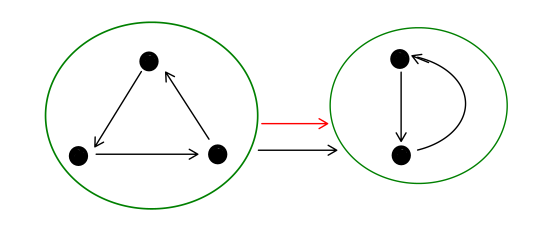
\includegraphics[width=5cm,height=4cm,keepaspectratio]{./Pictures/metagraph.png}\\

    Algorithmus von Kosaraju
    \begin{enumerate}
        \item Bestimme die reverse post-order (Alg. siehe oben)
        \item Bilde den transponierten Graphen $G^T$ (transpose\_graph() $\Rightarrow$ erste VL über Graphen)
        \item Bestimme die Zusammenhangskomponenten von $G^T$ mittels Tiefensuche ($\widehat{=}$ transitive Hülle der Anker), aber \emph{nicht} in der Reihenfolge der Knotenindizes, sondern in reverse post-order [for node in range(len(graph)): $\Rightarrow$ for node in rev\_post\_order:]
    \end{enumerate}

